\documentclass{article}
\usepackage[utf8]{inputenc}
\usepackage[sfdefault,ultralight]{FiraSans} %% option 'sfdefault' activates Fira Sans as the default text font
\usepackage[T1]{fontenc}
\renewcommand*\oldstylenums[1]{{\firaoldstyle #1}}
\usepackage{appendix}
\usepackage{graphicx}
\usepackage{amsfonts}
\usepackage{amssymb}
\usepackage{xcolor}
\usepackage{fdsymbol}
\usepackage{wasysym}
\usepackage{multicol}
\usepackage{amsmath,seqsplit}
\usepackage{algorithm, algorithmic}
\usepackage{tcolorbox}
\usepackage{geometry}
 \geometry{
 a4paper,
 right=20mm,
 left=25mm,
 top=25mm,
 bottom=25mm,
 }
\usepackage{pgfplots}
\usepackage{hyperref}
\usepackage{tikz}
\newcommand\foo[2]{%
    \begin{minipage}{#1}
    \seqsplit{#2}
    \end{minipage}
}

\setlength{\columnsep}{1cm}
\setlength\parindent{0pt}

\usepackage{tkz-graph}

\hypersetup{
  colorlinks=true,
  linkcolor=blue,
  urlcolor=blue,
}

\definecolor{pink}{RGB}{244,194,194}
\definecolor{green}{RGB}{143,188,143}
\definecolor{red}{RGB}{190,0,50}
\definecolor{ttgrey}{rgb}{0.58,0.59,0.69}
\definecolor{ttblue}{rgb}{0.2,0.17,0.38}
\definecolor{ttred}{rgb}{0.67,0.07,0.32}

\begin{document}

\begin{tcolorbox}[colframe=ttblue, colback=ttblue!10]
\begin{center}
\begin{large}
\textbf{Second homework Joosep Parts 221963IVCM}
\end{large}
\end{center}
\end{tcolorbox}

\section{Task}%1
Given the instantiation of Feistel network:
\begin{itemize}
  \item Block size = 16
  \item Number of rounds = 6
  \item Round function: $F(k_i, x) = k_i \oplus x$
  \item Key generation: $k_{i+1} = k_i \oplus \text{bin}(i+1)$ where $\text{bin}(i+1)$ is the binary representation of $(i + 1)$.
\end{itemize}

To encrypt the message $m = 0110\ 1001\ 1010\ 1111$ using the key $k_0 = 0101\ 1001$, we split the message into two halves, $L_0 = 0110\ 1001$ and $R_0 = 1010\ 1111$.

Using the round function and the key generation function, the encrypted message after 6 rounds of Feistel is calculated as:

\[ C = L_6 R_6 \]
\[ L_i = R_{i-1} \]
\[ R_i = L_{i-1} \oplus F(R_{i-1}, k_i) \]
\[ k_i = k_{i-1} \oplus \text{bin}(i) \]

After 6 rounds, the encrypted message is:

\[ C = 0110\ 1100\ 1010\ 1000 \]

\begin{verbatim}
[1] iteration 0 is: 1010 1111 1001 1111
[1] iteration 1 is: 1001 1111 0110 1000
[1] iteration 2 is: 0110 1000 1010 1101
[1] iteration 3 is: 1010 1101 1001 1100
[1] iteration 4 is: 1001 1100 0110 1100
[1] iteration 5 is: 0110 1100 1010 1000
[1] answer is: 0110 1100 1010 1000
\end{verbatim}

Proof can be seen in code: \href{https://stackblitz.com/edit/js-ekqepc?devtoolsheight=80&file=hw21.js&hideDevTools=false}{\texttt{stackblitz hw21}}\\
Code is also in repository: \href{https://github.com/Nurech/js-ekqepc}{\texttt{here}}

\section{Task}%2
Using the Vigenère cipher to encrypt the plaintext "THEWANDCHOOSESTHEWIZARD" with key "MAGIC", we get:
\begin{gather*}
    C = \text{{FHKECZDIPQASKAVTECQBMRJ}}\\
    C' = \text{{FHKECZDIPQASKAVTERQBMRJ}}\\
\end{gather*}

Diffusion: let's denote the original ciphertext as \( C \) and the modified ciphertext (after changing one letter in the plaintext) as \(
C' \).
The number of different characters between \( C \) and \( C' \) can be represented as the function \( \Delta(C, C') \).
Thus, for our given texts:
\[ \Delta(C, C') = n \]
where \( n \) is the number of letters that changed in the ciphertext due to the modification in the plaintext.
The limited value of \( n=1 \) suggests limited diffusion in the Vigenère cipher for this example.

\begin{gather*}
    C = \text{{FHKECZDIPQASKAVTECQBMRJ}}\\
    C'' = \text{{FHRECZDPPQASRAVTEJQBMRQ}}\\
\end{gather*}
Confusion: let's denote the ciphertext produced with the modified key as \( C'' \).
The number of different characters between \( C \) and \( C'' \) can be represented as:
\[ \Delta(C, C'') = m \]
where \( m \) is the number of letters that changed in the ciphertext due to the modification in the key.
Key is now \( MANIC \) instead of \( MAGIC \).
A relatively larger value of \( m=5 \) suggests \('\)better\('\) confusion in the Vigenère cipher for this example, however
I would say the statistical properties have not change much regardless of the key modification.\\

\begin{verbatim}
[2.1] Encrypted message: FHKECZDIPQASKAVTECQBMRJ
[2.2] Letter C changed to R at index 17
[2.2] modifiedPlainText: THEWANDCHOOSESTHELIZARD
[2.2] modifiedEncryptedText: FHKECZDIPQASKAVTERQBMRJ
[2.2] letters changed: 1
[2.3] Letter K changed to R at index 2
[2.3] Letter I changed to P at index 7
[2.3] Letter K changed to R at index 12
[2.3] Letter C changed to J at index 17
[2.3] Letter J changed to Q at index 22
[2.3] Key: MAGIC
[2.3] Encrypted with original key: FHKECZDIPQASKAVTECQBMRJ
[2.3] Modified key: MANIC
[2.3] Encrypted with modified key: FHRECZDPPQASRAVTEJQBMRQ
[2.3] Letters changed after modifying key: 5
\end{verbatim}


Proof can be seen in code: \href{https://stackblitz.com/edit/js-ekqepc?devtoolsheight=80&file=hw22.js&hideDevTools=false}{\texttt{stackblitz hw22}}\\
Code is also in repository: \href{https://github.com/Nurech/js-ekqepc}{\texttt{here}}

\section{Task}%3

For example, I take random key and two message parts and apply them.
For the function 1:
\begin{align*}
  \text{Given } m &= \text{"THEWAND"}, \\
  F'(k, m) &= F(k, \text{"THEWAND"}) \parallel 0^7 \\
  &= \text{"FHKECZD"} \parallel \text{"0000000"} \\
  &= \text{"FHKECZD0000000"}
\end{align*}

When appending 0's at the end of the function makes it predictable as we can see it's not completely indisdinguishable from totally
random function.\\

For the function 2:

\begin{align*}
  \text{Given } m_1 &= \text{"THEWAND"}, \\
  m_2 &= \text{"CHOOSER"}, \\
  F'(k, m_1 \parallel m_2) &= F(k, \text{"THEWAND"}) \parallel F(k, \text{"CHOOSER"}) \oplus \text{"0000000"} \\
  &= \text{"FHKECZD"} \parallel \text{"LFHBL"} \\
  &= \text{"FHKECZDLFHBL"}
\end{align*}

For this the XOR with 0's does not change m2, so it's better but the security depends on the security of the function F.
So it's not completely secure but better than function from task 1.

For the function 3:

\begin{align*}
  \text{Given } m_1 &= \text{"THEWAND"} \text{ and } m_2 = \text{"CHOOSER"}, \\
  F'(k, m_1 \parallel m_2) &= F(k, \text{"0THEWAND"}) \oplus F(k, \text{"CHOOSER1"}) \\
  \text{Result} &= \text{""}
\end{align*}
Text is in hex, so it's not readable. 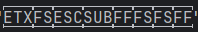
\includegraphics{img}
This XOR operation provides a more randomized and harder-to-predict output, given two distinct inputs.
So in my opinion this is the best function of the three and attacker would guess this with more than $\frac{1}{2}$  probability.\\

\begin{verbatim}
[3.1] Using F'(k, m) = F(k, m)||0^n
[3.1] Message: THEWAND
[3.1] Key: MAGIC
[3.1] Result: FHKECZD0000000
[3.2] Using F'(k, m1||m2) = F(k, m1)||F(k, m2 ⊕ 0^n)
[3.2] Message 1: THEWAND
[3.2] Message 2: CHOOSER
[3.2] Key: MAGIC
[3.2] Result: FHKECZDLFHBL
[3.3] Using F'(k, m1||m2) = F(k, 0||m1) ⊕ F(k, m2||1)
[3.3] Message 1: THEWAND
[3.3] Message 2: CHOOSER
[3.3] Key: MAGIC
[3.3] Result: 
\end{verbatim}

Proof can be seen in code: \href{https://stackblitz.com/edit/js-ekqepc?devtoolsheight=80&file=hw23.js&hideDevTools=false}{\texttt{stackblitz hw23}}\\
Code is also in repository: \href{https://github.com/Nurech/js-ekqepc}{\texttt{here}}

\section{Task}%4

\subsection*{4.1: Encryption using Permutation Cipher in OFB Mode}

Given:
\begin{align*}
  D &= 00011 \\
  O &= 01110 \\
  G &= 00110 \\
\end{align*}

Thus, the plaintext in binary is:
\[
  P = 00011\,01110\,00110
\]

For the OFB mode with key \( K = (4,1,3,5,2) \):

\begin{align*}
  1. &\text{ IV } w = 01011 \rightarrow \text{Permute to get } 10011 \\
  2. &\text{ XOR } P_1 \text{ with IV to get } C_1: 00011 \oplus 10011 = 10000 \\
  3. &\text{ Continue for } P_2, P_3 \text{ to get } C_2, C_3
\end{align*}

Resulting in:
\[
  C = 10000\,10100\,11111
\]

\subsection*{4.2: Decryption with Modified Ciphertext}

Flipping the 5-th bit of \( C \):
\[
  C' = 10001\,10100\,11111
\]
Decryption yields:
\[
  P' = 00010\,01110\,00110
\]
Differing from \( P \) by 1 bit.

\subsection*{4.3: Decryption with Modified IV}

Using the modified IV \( w' = 11011 \), decryption provides:
\[
  P'' = 01011\,01111\,00100
\]
This differs from \( P \) by 3 bits.\\

\begin{verbatim}
[4] Binary Plaintext D: 00011 O: 01110 G: 00110
[4] After Permutation (using key): 10011
[4] XOR of Plaintext block: 00011 with iv: 10011 and get EncBlock: 10000
[4] After Permutation (using key): 11010
[4] XOR of Plaintext block: 01110 with iv: 11010 and get EncBlock: 10100
[4] After Permutation (using key): 11001
[4] XOR of Plaintext block: 00110 with iv: 11001 and get EncBlock: 11111
[4.1] Encrypted Ciphertext: 10000 10100 11111
[4.2] Modified Ciphertext by flipping 5-th bit: 100011010011111
[4.2] Decrypted Binary for modified Ciphertext: 000100111000110
[4.2] originalBinaryPlaintext: 000110111000110
[4.2] decryptedBinary2: 000100111000110
[4.2] changedBits2: 1
[4.3] Decrypted Binary using modified IV: 010110111100100
[4.3] decryptedBinary3: 010110111100100
[4.3] originalBinaryPlaintext: 000110111000110
[4.3] Number of bits changed in plaintext for: 3
\end{verbatim}

Proof can be seen in code: \href{https://stackblitz.com/edit/js-ekqepc?devtoolsheight=80&file=hw2_4.js&hideDevTools=false}{\texttt{stackblitz hw24}}\\
Code is also in repository: \href{https://github.com/Nurech/js-ekqepc}{\texttt{here}}

\section{Task}%5


\begin{tikzpicture}
    % Nodes
  \node (iv) {IV: $r_0$};
  \node [below of=iv, node distance=2cm] (m1) {$m_1$};
  \node [below of=m1, node distance=2cm] (m2) {$m_2$};
  \node [below of=m2, node distance=2cm] (mn) {$m_n$};
  \node [right of=iv, node distance=3cm] (e1) {$E(k, m_1)$};
  \node [below of=e1, node distance=2cm] (e2) {$E(k, m_2)$};
  \node [below of=e2, node distance=2cm] (en) {$E(k, m_n)$};
  \node [right of=e1, node distance=3cm] (c1) {$c_1$};
  \node [below of=c1, node distance=2cm] (c2) {$c_2$};
  \node [below of=c2, node distance=2cm] (cn) {$c_n$};

  % Paths
  \path [->] (iv) edge (e1);
  \path [->] (m1) edge (e1);
  \path [->] (m2) edge (e2);
  \path [->] (mn) edge (en);
  \path [->] (e1) edge node[above] {$\oplus$} (c1);
  \path [->] (c1) edge (e2);
  \path [->] (e2) edge node[above] {$\oplus$} (c2);
  \path [->] (c2) edge (en);
  \path [->] (en) edge node[above] {$\oplus$} (cn);
\end{tikzpicture}
\subsection*{Decryption Process}

XOR is its own inverse, so the decryption process is almost identical to the encryption process but in reverse order.
To decrypt you would do the following:

\begin{tikzpicture}
  % Nodes
  \node (iv) {IV: $r_0$};
  \node [below of=iv, node distance=2cm] (c1) {$c_1$};
  \node [below of=c1, node distance=2cm] (c2) {$c_2$};
  \node [below of=c2, node distance=2cm] (cn) {$c_n$};
  \node [right of=iv, node distance=3cm] (d1) {$D(k, c_1)$};
  \node [below of=d1, node distance=2cm] (d2) {$D(k, c_2)$};
  \node [below of=d2, node distance=2cm] (dn) {$D(k, c_n)$};
  \node [right of=d1, node distance=3cm] (m1) {$m_1$};
  \node [below of=m1, node distance=2cm] (m2) {$m_2$};
  \node [below of=m2, node distance=2cm] (mn) {$m_n$};

  % Paths
  \path [->] (iv) edge (d1);
  \path [->] (c1) edge (d1);
  \path [->] (c2) edge (d2);
  \path [->] (cn) edge (dn);
  \path [->] (d1) edge node[above] {$\oplus$} (m1);
  \path [->] (m1) edge (d2);
  \path [->] (d2) edge node[above] {$\oplus$} (m2);
  \path [->] (m2) edge (dn);
  \path [->] (dn) edge node[above] {$\oplus$} (mn);
\end{tikzpicture}
\subsection*{Decryption Process}



\section{Task}%6

\subsection*{6.1: Output each integer five times}
Given that one output operation takes a constant amount of time (let's call this constant \(c\)), for \(n\) integers, outputting each 5 times will take \(5nc\) time.

\begin{align*}
  \text{Time for 1} & : 5nc = c \times O(n) = O(n)
\end{align*}

\subsection*{6.2: Apply bubble sort}
In bubble sort, we repeatedly traverse the array and swap adjacent elements if they are in the wrong order. The worst-case occurs when the array is reverse sorted, which requires \(\frac{n(n-1)}{2}\) comparisons and swaps.
Let's take a simple reversed array of size 4 for illustration: \( \{4, 3, 2, 1\} \)

\begin{itemize}
  \item \textbf{1\textsuperscript{st} pass}: Compare 4 and 3, 3 and 2, 2 and 1. 3 swaps. Array becomes \( \{3, 2, 1, 4\} \)
  \item \textbf{2\textsuperscript{nd} pass}: Compare 3 and 2, 2 and 1. 2 swaps. Array becomes \( \{2, 1, 3, 4\} \)
  \item \textbf{3\textsuperscript{rd} pass}: Compare 2 and 1. 1 swap. Array becomes \( \{1, 2, 3, 4\} \)
\end{itemize}

\begin{align*}
  \text{Time for 2} & : \frac{n(n-1)}{2} = O(n^2)
\end{align*}

\subsection*{6.3: Find greatest common reminder of 2\textsuperscript{nd} and 4\textsuperscript{th} elements of the array}
The operation of fetching two fixed positions (like 2\textsuperscript{nd} and 4\textsuperscript{th} elements) is \(O(1)\), as array
access is instant.
The Euclidean algorithm's time complexity for GCD is roughly proportional to the number of digits of the smaller number.
The number of steps to calculate the GCD of two natural numbers, \(a\) and \(b\), may be denoted by \(T(a, b)\). If \(g\) is the GCD of \(a\) and \(b\), then \(a = mg\) and \(b = ng\) for two coprime numbers \(m\) and \(n\).
Hence,
\begin{align*}
  T(a, b) = T(m, n)
\end{align*}

The recursive nature of the Euclidean algorithm yields:
\begin{align*}
  T(a, b) & = 1 + T(b, r_0) \\
  & = 2 + T(r_0, r_1) \\
  & \vdots \\
  & = N + 1
\end{align*}
where \(T(x, 0) = 0\) by assumption.

Worst case explanation taken from \href{https://en.wikipedia.org/wiki/Euclidean_algorithm#Algorithmic_efficiency}{\texttt{wikipedia}}, also
tells us that Euclidean algorithm always requires fewer than \(O(h)\) divisions, where \(h\) is the number of digits in the smaller
number \(b\). since $O(1) < O(b)$ O complexity is:

\begin{align*}
  \text{Time for Step 3} & : O(b)
\end{align*}


\section{Task Bonus}
OTP (One Time Pad) encryption, when used correctly, provides perfect secrecy.
However, when applied in CBC mode, its properties change.
In CBC mode, each block of plaintext is XORed with the previous ciphertext block before being encrypted with the OTP.
The first block of plaintext is XORed with an initialization vector (IV).
Thus, if an adversary knows one plaintext block and its corresponding ciphertext block, he can infer information about the next plaintext block.
Code encrypts both \(m_0\) and \(m_1\) in CBC mode using OTP.
Then, the adversary attacks by computing the encryption of \(m_0\) and
comparing it with the received ciphertext to infer which message was encrypted first.

\begin{verbatim}
[BONUS] m0 string: Hello
[BONUS] m1 string: World
[BONUS] key: supersecretkey
[BONUS] iv: 12345
[BONUS] otpCbcEncrypt with: Hello+World supersecretkey 12345
[BONUS] CipherText:"/=(.(>#)
[BONUS] cipherM0:"/=(
[BONUS] cipherText.slice(0, iv.length):"/=(
[BONUS] m0(1st block) has been encrypted.
\end{verbatim}

Proof can be seen in code: \href{https://stackblitz.com/edit/js-ekqepc?devtoolsheight=80&file=bonus.js&hideDevTools=false}{\texttt{stackblitz bonus}}\\
Code is also in repository: \href{https://github.com/Nurech/js-ekqepc}{\texttt{here}}

\end{document}
